\documentclass[10pt]{article}
\usepackage[english]{babel}
\usepackage[utf8]{inputenc}
\usepackage[OT1]{fontenc}
\usepackage{amsfonts, amsmath, amsthm, amssymb}
\usepackage{graphicx}
\usepackage{listings}
\usepackage[margin=1in]{geometry}
\usepackage{brad}


\title{Using the Gauss-Bonnet Theorem}
\author{Bradley McCoy}
\date{\today}
\begin{document}
\maketitle \tableofcontents 

\section{Preface}

Using the borsuk-ulam theorem rules \cite{jm08}.
Several applications are given in do Carmo \cite{doc76}.
We highlight a subset of these.











\section{Manifolds, Curvature, and the Euler Characteristic}
\label{sec:cast}


The Gauss-Bonnet theorem is a bridge. On one shore is topology and
on the opposite shore geometry. This bridge can be traveled in both directions.
That is, if one has geometric information one can deduce topological information and
if one has topological information one can deduce geometric information.
In symbols, the theorem can be stated as follows

\begin{equation} \label{eqn:g-b}
\int_M K dA + \int_{\partial M} k_g ds = 2\pi \chi(M).
\end{equation}
In this section, we define these symbols.

\subsection{Preliminaries}

We begin with some definitions a that may already be familiar to the reader,
\begin{definition}[Topological Space \cite{munkres}]
A \EMPH{topology} is a pair $(X,\tau)$, where $X$ is a set and
 $\tau$ is a collection of subsets $X$
satisfying:
	\begin{itemize}
		\item $\emptyset$ and $X$ are in $\tau.$
		\item the union of \emph{any} subcollection of elements in $\tau$ is  in $\tau.$
		\item the intersection of any \emph{finite} subcollection of elements in the $\tau$ is in $\tau.$
	\end{itemize}
A set $X$ with a specified topology $\tau$ is called a \EMPH{topological space}.
\end{definition}

We will work with a special type of topological spaces called manfiolds.

\begin{definition}[Manifold  \cite{tu2011}]
	A topological space $M$ is \EMPH{locally Euclidean of dimension $n$}
	if every point $p$ in $M$has a neighborhood $U$ such that there is  a
	homeomorphism  $\phi$ from $U$ into and open  subset of $\R^n$.
	We call the pair $(U,\phi: U\to \R^n)$ a \EMPH{chart}, $U$ a \EMPH{coordinate neighborhood}
	and  $\phi$ a \EMPH{coordinate map}. 
A \EMPH{manifold} is a Hausdorff, second countable, locally Euclidean space.
\end{definition}

The symbol $M$ in \eqnref{g-b} is a manifold. For the most part, we will consider two dimensional manifolds that are called \emph{surfaces}.
We will consider both continuous and discrete objects.
For computational purposes, we often want a combinatorial structure on our manifolds.
This structure will often come in the form a triangulation, which we now define.


\begin{definition}[Independent Points]
Let $v_0,v_1,\ldots,v_k$ be points in $\R^n$. We call them \EMPH{affinely dependent}
if there are real numbers $\alpha_0,\alpha_1,\ldots,\alpha_k$, not all 0, such that
$\Sigma_{i=0}^k \alpha_iv_i=0$ and $\Sigma_{i=0}^k \alpha_i=0.$
Otherwise,  $v_0,v_1,\ldots,v_k$ are \EMPH{affinely independent}.

\end{definition}

\begin{definition}[Simplices]
A \EMPH{simplex} $\sigma$ is the convex hull of a finite affinely independent
set $A$ in $\R^n$. The points in  $A$ are  called vertices, the dimension
of  $\sigma$ is $|A|-1$.  The convex hull of a subset of vertices of a simplex
$\sigma$ is a \EMPH{face} of $\sigma$.
\end{definition}

\begin{definition}[Simplicial Complex]
A nonempty family $C$ of simplices is a \EMPH{simplicial complex} if the following
are satisfied:
\begin{itemize}
\item  Each face of any simplex is a simplex.
\item The intersection of $\sigma_1 \cap \sigma_2$ is a face of both $\sigma_1$ and 
$\sigma_2$.
\end{itemize}


\end{definition}

For many of our applications we will consider a special type of manifold called
a triangular mesh. Meshes are used extensively in graphics.


\begin{definition}[Homeomorphism]
A  \EMPH{homeomorphism}  of topological spaces $(X_1,\tau_1$ and $(X_2,\tau_2)$
is a bijection $\phi:X_1\to X_2$ such that for every $\phi$ and $\phi^{-1}$ are continuous.
\end{definition}
For two topological spaces $X$ and $Y$ if there exists a  homeomorphism between
$X$ and $Y$ we say $X$ and $Y$ are topologically  equivalent and write  $X\cong Y.$

\begin{definition}[Triangulation]
For a topological space $X$ and simplicial complex $C$ if $X\cong C$,
then $C$  is a \EMPH{triangulation} of $X$.
\end{definition}

Often, it is useful to approximate smooth surfaces with fine triangulations called
a \emph{mesh}. We will see meshes in many of our applications.

\subsection{Curvature}

Continuous:

For a curve in $\R^3$ how can we quantify the curvature at a point on the curve?
Let $\gamma$ denote a curve in $\R^3$ and let $p$ be a point on $\gamma$.
We traverse $\gamma$ at unit speed, $\gamma(t)=(x(t),y(t),z(t))$.  
Let $\vec{T}$ denote the unit tangent vector of $\gamma$ at $p$. 
The curvature is how much the tangent vector $\vec{T}=(x'(t),y'(t),z'(t))$ is rotating. 
This is exactly the second derivative $\gamma''$. Since we traverse $\gamma$
at unit speed, $\gamma'(t)^2=1,$ and by the chain rule, $\gamma'\cdot \gamma''=0,$
so  the second derivative is orthogonal to $\gamma'$. The norm of the second
derivative is the curvature $k$.
Let $n$ denote a unit vector parallel to $\gamma''$, then $\gamma''=k n$.
By taking the cross product of $N$ and $T$ we obtain a vector $B$.
The vectors $T,N$ and $B$ form the \emph{Fernet frame} of $\gamma$ a $p.$


The curvature $k$ of a curve in $\R^3$ is equivalent to the inverse of the radius
of the circle that best approximates the curve at a point. This circle is called
the osculating circle. 
For example, the unit circle in the $xy$-plane, parameterized by $\gamma(t)=(\cos(t),\sin(t),0)$
we have $\gamma'(t)=(-\sin(t),\cos(t),0)$ and $\gamma''(t)=(-\cos(t),-\sin(t),0)$ and $||\gamma''||=1$
which agrees with the inverse of the radius of the osculating circle.
Another example is a straight line,
the curvature is zero and the radius of the osculating circle is infinite.

We will consider one-dimensional curves that are the boundary of two-dimensional
surfaces $S$ in $\R^3.$ In a surface, a \EMPH{geodesic} is a curve that is a shortest path
between two points in the surface. For example, on $\Sp^2$, the equator is a geodesic
and an inhabitant would view a geodesic as a straight line. 
Then, since $S$ is a manifold, each point has a local chart with a normal vector $N$.
We want to compute the rate of rotation of $\gamma$ about $N$.
We project $\gamma'$ onto the tangent plane to $S$ at $p$.
If $T$ is a unit length tangent vector at p, then the vector $U=N\times T$
is orthogonal to both $N$ and $T$.
The \EMPH{geodesic curvature} $k_g$ at a point $p$ is defined to be the norm of the projection
of $k$ onto the tangent space of $S$ at $p$. The geodesic curvature can be computed
by the formula $k_g(t)=||(\gamma''\cdot U)\cdot U||.$

In two-dimensions, we wish to calculate the rate at which the surface
pulls away from the tangent plane.  There are several equivalent ways 
to calculate curvature of a surface.
We can generalize the concept of an osculating circle to an
osculating sphere or we can compute the rate of change of
a normal vector at a point $p$.

Given a surface, we can define a normal vector on the surface at  a point
by considering a local coordinate chart at $p$ with axis $u$ and $v$.
Once we choose a chart we define a clockwise orientation. If the clockwise
orientation can be consistently extended to the entire surface, we say
the surface is \EMPH{orientable}.

For an orientable surface $S$, the map that  $N:S\to \Sp^2$ that sends each
normal in $S$ to the corresponding point on $\Sp^2$ is
the \EMPH{Gauss map}.
The derivative of the Gauss map, $dN(p)$ quantifies the rate of change of
the normal vector ($dN$ is often called the \emph{Weingarten map} \cite{Crane:2013}).
Thus, $dN_p:T_p(S)\to T_{N(p)}(\Sp^2)$, but since $T_p(S)$ and $T_{N(p)}(\Sp^2)$
are parallel we can define $dN_p$ to be a linear map on $T_p(S)$.

Discrete:

Recall that the sum of the interior angles of a triangle is $\pi$,
see \figref{angles} for proof. By induction, the sum of the interior angles
of a convex polygon with $n$ edges is  $(n-2)\pi$, see \figref{angles}
for an example. 

\begin{figure}[htb]
\centering
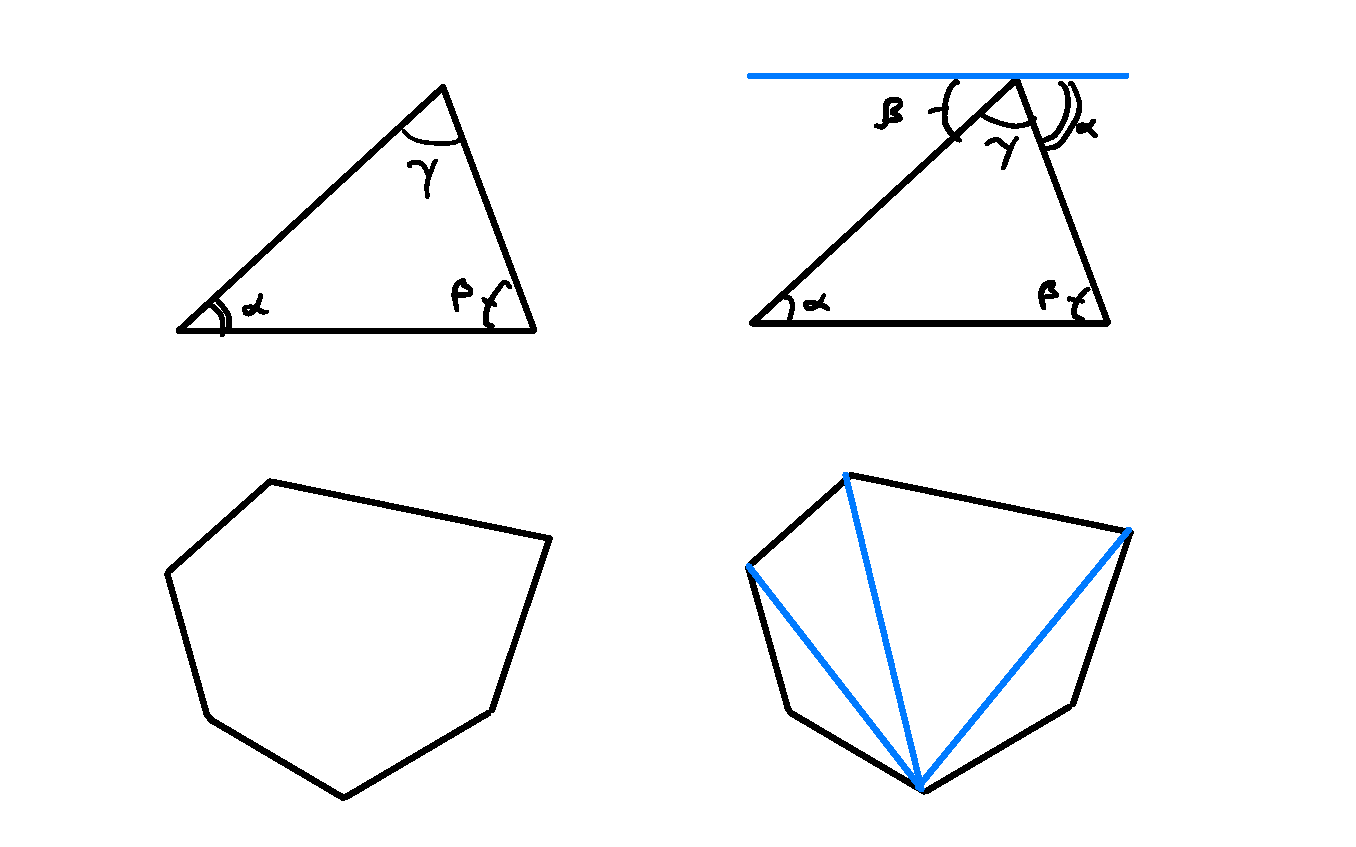
\includegraphics[width=.3\textwidth]{curvature/convex-angles}
\caption{Top row: the sum of  the interior angles of a triangle is $\pi$.
Bottom row: the sum of the interior angles of a convex polygon on $n$ edges is $(n-2)\pi$.}
\label{fig:angles}
\end{figure}


There are several ways to define curvature in the discrete setting \cite{Crane:2013},
this definition will be used in the poof of the discrete Gauss-Bonnet in \secref{proof}.

''For a discrete planar curve we can define the curvature at a vertex as the distance on the unit circle between the two adjacent normals'' \cite{Crane:2013}.

\begin{definition}[Discrete Gaussian curvature \cite{upadhyay2015}]\label{def:discrete-curvature-vertex}

The discrete \EMPH{Gaussian curvature} at a vertex $v$ is the area on the unit sphere bounded by a spherical polygon whose vertices are the unit normals of the faces around $v$.

\end{definition}


\begin{figure}[htb]
\centering
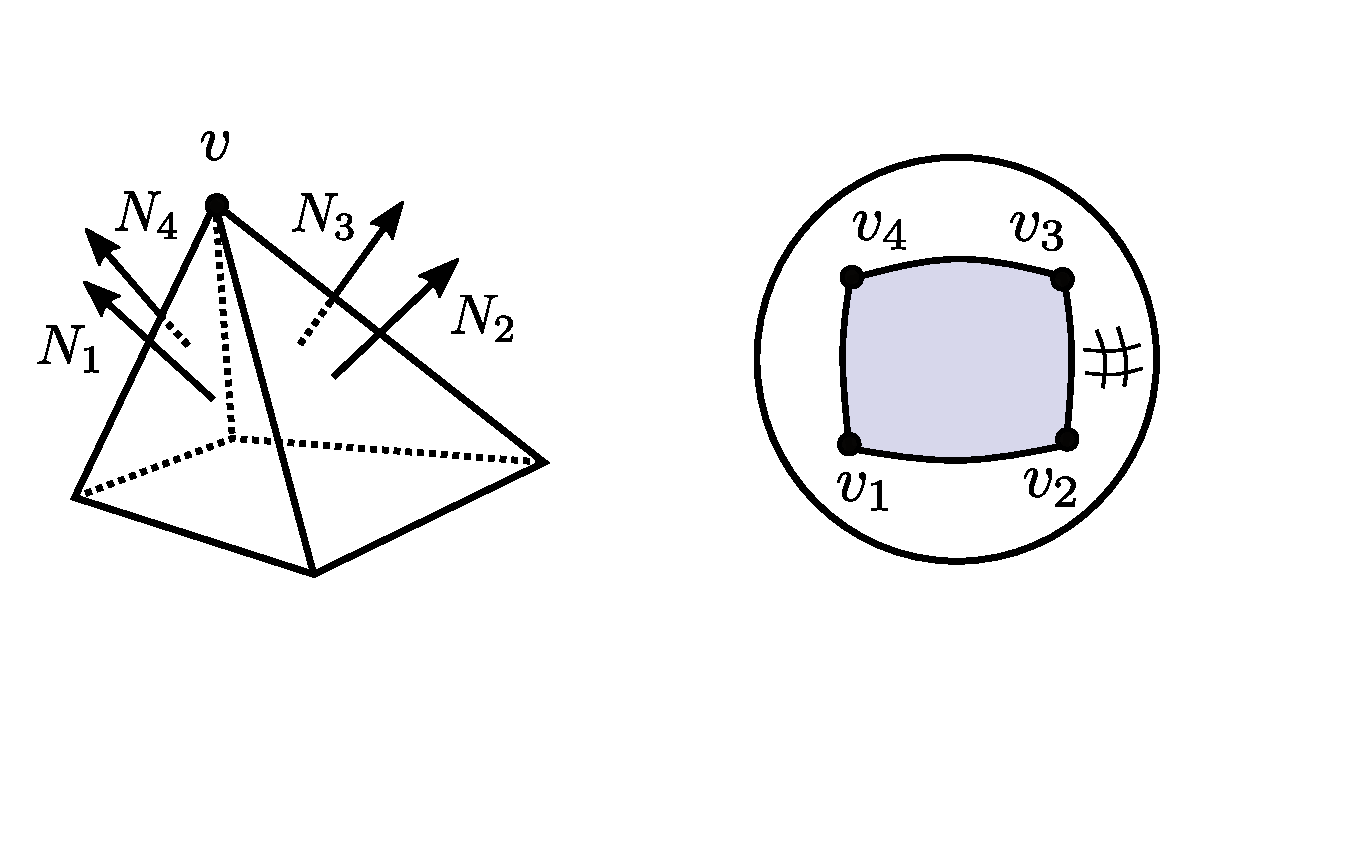
\includegraphics[width=.3\textwidth]{curvature/discrete-curvature}
\caption{The discrete curvature at vertex $v$ is the area drawn on the sphere.}
\label{fig:discrete-curvature}
\end{figure}

The \EMPH{angle defect} at a vertex $d(v)$ is the difference between $2\pi$ and
the sum of the incident angles.  Let $F_v$ denote the faces containing $v$  
and let $\alpha_f$  denote the interior  angle of face $f$ at $v$, then
$$d(v):=2\pi -\sum_{f\in F_v}\alpha_f.$$

The angle defect is equal to the discrete curvature in \defref{discrete-curvature-vertex}.

\subsection{The Euler Characteristic}

Properties of topological spaces that remain unchanged by homeomorphisms are called
\EMPH{topological invariants}. One such invariant is the Euler characteristic.
Originally defined for polyhedra, the \EMPH{Euler Characteristic} for surfaces $\chi$ is the 
the number of vertices minus the number of edges plus  the number of faces, $\chi=V-E+F.$
In higher dimensions, for a triangulated space $X$ the Euler characteristic is 
$\chi(X)=k_0-k_1+k_2-k_3+\ldots$ where $k_n$ is the number of simplices of dimension $n.$
A  graph  is \EMPH{planar} if it can be drawn in the plane with intersections only occuring
at vertices.
For a planar graphs $V-E+F=2$, Eppstein maintains a collection of proofs of this \cite{eppstein-proofs}.
We include the the following proof from Eppstein's list attributed to Thurston
 \cite{thurston}. For any planar graph we can map the graph on to the two sphere
 using stereographic projection.
 
\begin{theorem}[Euler Characteristic for Planar Graphs]\label{thm:euler}
For any planar graph on the 2-sphere we have $V-E+F=2.$
\end{theorem}

\begin{proof}
If needed, perturb the triangulation so that the north and south poles are 
inside of a two faces and there are no vertical edges. At each vertex place a unit positive
charge, at the center of each edge place a unit negative charge and put a unit positive
charge in the middle of each face. Slam the sphere on the ground so that all charges
on the edges and vertices are moved into the face below them. For faces that do not contain a pole
the net charge will be zero, the northern boundary consists of an alternating sequence
of edges and vertices  beginning  and ending with an edge.
The face containing the north pole has a unit positive charge, and the face containing the south
pole contains positive four units of charge and negative three units of charge.
Thus, the total charge is two.

\end{proof}

\subsection{A Combinatorial Proof}
\label{sec:proof}


We present a proof of the Gauss-Bonnet theorem similar to the proof given by Upadhyay \cite{upadhyay2015}.
First, we consider the case where our surface does not have a boundary.
We then extend this case to surfaces with boundary.
\begin{theorem}[Discrete surfaces without boundary]\label{thm:g-b-discete-bdy}
For a triangulated surface $S$ without boundary
$$\sum_{v\in V} K(v)=2\pi \chi(S)$$
where $K(v)$ is the discrete curvature.
\end{theorem}

\begin{proof}

For each vertex $v$ in $S$,
let $deg(v)$ denote the number of edges incident to $v$, let $\alpha_1,\alpha_2,\ldots,\alpha_{\deg{(v)}}$ denote the angles
containing $v$ and let $\xi_i=\pi-\alpha_i$ for each $i$.
By \eqnref{discrete-curvature-complement-angle}, 
the discrete Gaussian curvature at a $v$ is
 $$K(v)=(2-\deg{(v)})\pi +\sum_{i=1}^{\deg{(v)}} \xi_i.$$
Summing over all vertices in $S$ gives
$$\sum_{v\in V} K(v)=\sum_{v\in V}2\pi - \sum_{v\in V}\deg{(v)}\pi+\sum_{v\in V}\sum_{i=1}^{\deg{(v)}} \xi_i.$$
The first term on the right hand side is $2\pi |V|$. Each edge is incident with two vertices, so the second term is $2\pi |E|$. 
In the third term, we rewrite $\xi_i$ as $\pi-\alpha_i$.

$$ \sum_{v\in V}\sum_{i=1}^{\deg{(v)}} \beta_i= \sum_{v\in V}\sum_{i=1}^{\deg{(v)}} (\pi-\alpha_i).$$
We can reorganize this sum as follows, instead of summing the angles around each vertex we can sum the angles in each face.
Each angle in $S$ is still being counted exactly once. 
Since each face is a triangle, this gives
$$\sum_{v\in V}\sum_{i=1}^{\deg{(v)}} (\pi-\alpha_i)=\sum_{f\in F}\sum_{i=1}^3(\pi-\alpha_i).$$
Since each face is a triangle the sum of the three angles is $\pi$,
so $\sum_{i=1}^3(\pi-\alpha_i)=3\pi-\pi=2\pi.$
Thus, $$\sum_{v\in V} K(v)=2\pi |V|-2\pi |E|+2\pi |F|=2\pi \chi(S)$$ as desired.
\end{proof}

Next, we extend the above proof to the case where $S$ has a boundary
by gluing a copy of $S$ to itself along the boundary.

\begin{theorem}[Discrete surfaces without boundary]\label{thm:g-b-discete}
For a combinatorial surface $S$ with boundary

$$\sum_{v\in S_{\text{int}}} K(v)+\sum_{v\in\partial S}k_g(v)=2\pi \chi(S)$$
where $K(v)$ is the discrete curvature and $k_g(v)$ is the discrete geodesic curvature.
\end{theorem}

\begin{proof}
Take a copy of $S$ and attach it to itself along the boundary.
This creates the surface $2S$ without boundary. Notice,
when we copy $S$ we create two copies of the boundary, and when
we glue we remove one copy of the boundary.
Thus, $$\chi(2S)=2\chi(S)-\chi(\partial S).$$
Since, $\partial S$ is piecewise linear the number of vertices and
edges are equal and there are no faces, so $\chi(\partial S)=0$
and 

\begin{equation} \label{eqn:glue}
\chi(2S)=2\chi(S).
\end{equation}
For $v$ a vertex on the boundary, $k_g(v)$ is half
the discrete Gaussian curvature of $v$ in $2S.$
Thus,

$$\sum_{v\in 2S}K(v)=2\left(\sum_{v\in S_{\text{int}}}K(v)+\sum_{v\in \partial S} k_g(v)\right) =2\pi  \chi(2S).$$
Applying \eqnref{glue},

$$\sum_{v\in S}K(v)+\sum_{v\in \partial S} k_g(v)=2\pi  \chi(S)$$
as desired.

\end{proof}
\section{Applications}\label{sec:applications}
\section{Removing Noise From A Scanned Object}
\label{sec:removing}



Meshes that are obtained by scanning real objects contain noise.
Most meshes that are generated by scanning require a complete
remeshing \cite{remeshing-2003}.
As a first step in remeshing, the curvature at each
vertex needs to be estimated.

In \cite{mmsb-2003}, Meyer et al., define the gaussian curvature operator
to estimate the curvature at each vertex. Their operator is 
based on a simple application of the Gauss-Bonnet theorem.
The central idea is to cut a disk around each vertex that does not contain
any other vertices. Then, all Gaussian curvature in the removed
disk is occurs at the vertex of interest.

We associate an area around each vertex$v$. 
For each triangle incident to $v$, if the interior 
angle at $v$ is non-obtuse, mark the circumcenter of the triangle
and if the interior angle is obtuse, make the mid point of the edge
opposite of $v$. See \figref{mixed-area} for an illustration.
Denote the area of this polygon by $A_m.$


\begin{figure}[htb]
\centering
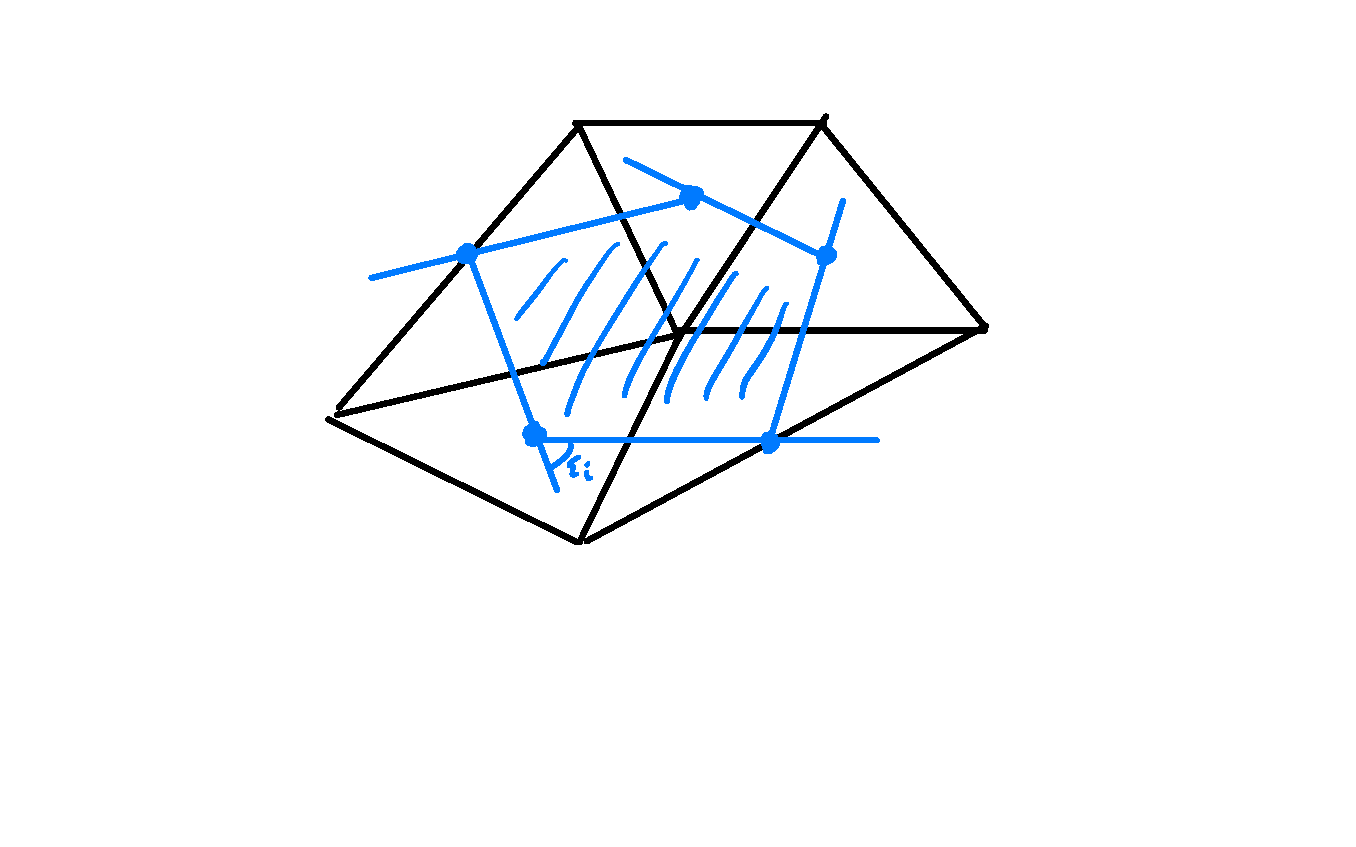
\includegraphics[width=.3\textwidth]{meshes/mixed-area}
\caption{The area $A_m$ associated with a vertex $v$.}
\label{fig:mixed-area}
\end{figure}


Then, since we are considering a closed two-disk $A$ we have $\chi(A)=1$.
Let $F_v$ denote the number of faces incident to $v$, 
then by the Gauss-Bonnet theorem we have

$$\int \int_{A_m}K dA +\sum_i^{F_v} \epsilon_i=2\pi$$
where the sum is over the faces incident to $v$.
The Gaussian curvature operator at a vertex $v$ is defined
to be
$$K(v)=\left( 2\pi -\sum_i^{F_v}\epsilon_i\right)/ A_m.$$

The experiments in \cite{mmsb-2003} found that the average
percent error did not exceed $1.3\%$ when using this operator.


\subsection{Robotics}
\label{sec:robotics}
In may 2023 I asked chatgbt to give me some applications of the Gauss-Bonnet theorem and returned
that there were applications to robotics. I asked for some references it gave me references
that were made up. But the suggestion lead me to the following
not made up application of the Gauss-Bonnet theorem in robotic 
route planning is given by K.-L. Wu et. al. in \cite{wu_path_2016}.
Suppose have a robot navigating a 3D\todo{2 or 3 manifold?} terrain with a single obstacle
and we wish to plan trips for our robot.
In this application, a terrain is a smooth manifold \todo{not defined} with tangent planes
at every point. An obstacle is modeled by a hazardous ball with a grade depending on the radius.
Assume that checking if a path intersects the obstacle can be done in constant time.


Overview of their procedure.
We are given two points $s$ and $t$ on a ?-manifold $M$.
First, compute a geodesic path from  $s$ to $t$ call this path $\gamma(x)$.
If the $\gamma$ does not intersect the obstacle we are done.
Otherwise, the $\gamma$ intersects the obstacle
we call the initial intersection point between our path
and the boundary of the obstacle $p$.
Construct the tanged plant $TpM$ at $p$.
Choose a vector $v\in TpM$ and a value $\alpha$ for the magnitude of $v$.
Next, define two points $\alpha_{\ell}$ and $\alpha_{u}$
to be in the directions of $v$ and $-v$ at a distance of $\alpha$
from $p$ in the tangent plane. Then project the points   $\alpha_{\ell}$ and $\alpha_{u}$
onto the surface? to obtain the points $q$ and $r$.
We next compute four new  geodesics $g_1(s)$ from $s$ to $q$,
$g_2(s)$ from $q$ to $t$, 
$f_1(s)$ from $s$ to $r$ and 
$f_2(s)$ from $r$ to $t$. Let $\gamma_g=g_2\circ g_1$ and $\gamma_f=f_2\circ f_1$.

We then use the Gauss-Bonnet theorem to decide which alternative path is best.
If the edges of a triangle are all geodesic then we have a \EMPH{geodesic triangle} $\tau\subset M$.
We have two geodesic triangles, $\gamma, g_1,g_2$ and $\gamma,f_1,f_2.$

Here we have cusps at the intersection points of the geodesics,
to account for this, our Gauss-Bonnet is 
\begin{equation}\label{eqn:b-g-angles}
\int \int_{\tau} K dA +\sum_{i=1}^3(\pi-\theta_i)+\sum_{i=1}^3 \int k_gds =2\pi
\end{equation}
where $\theta_i$ are the interior angles of $\tau$.
Since we are on geodesics $\int kgds =0$ and we can rearrange
\eqnref{b-g-angles} to obtain

\begin{equation} \label{eqn:interior-angles}
\theta_1+\theta_2+\theta_3 = \pi +\int \int_{\tau} K dA.
\end{equation}

We can estimate the curvature based on the sum of the angles of
$\sum_{i=1}3\theta$.
They show that f $K=0$ on $\tau$ then $\gamma_f$ and $\gamma_g$
are identical and there exists an $\alpha^*$ that makes them shortest.
If $\sum_{i=1}^3\theta_i>\pi$ then is $\int_?K>0$ on all of $\tau$ then and if $\sum_{i=1}^3\theta_i<\pi$
then $K<0$ on (average) all of $\tau$.
The authors state that we should avoid negative curvature because it
is ``energy-consuming ascending and descending motions required"
and would require the robot have ``better mobility and maneuverability".
\todo{I don't see why}.



\section{How Many Deltahedron Exist?}
\label{sec:deltahedron}

In this section, we share a proof due to
Fushsida-Hardy \cite{deltahedron} that there are
only eight deltahedron.

A \EMPH{deltahedron} is a polyhedron whose
faces are all equilateral triangles. Two examples are shown
in \figref{deltahedron}.


\begin{figure}[htb]
\centering
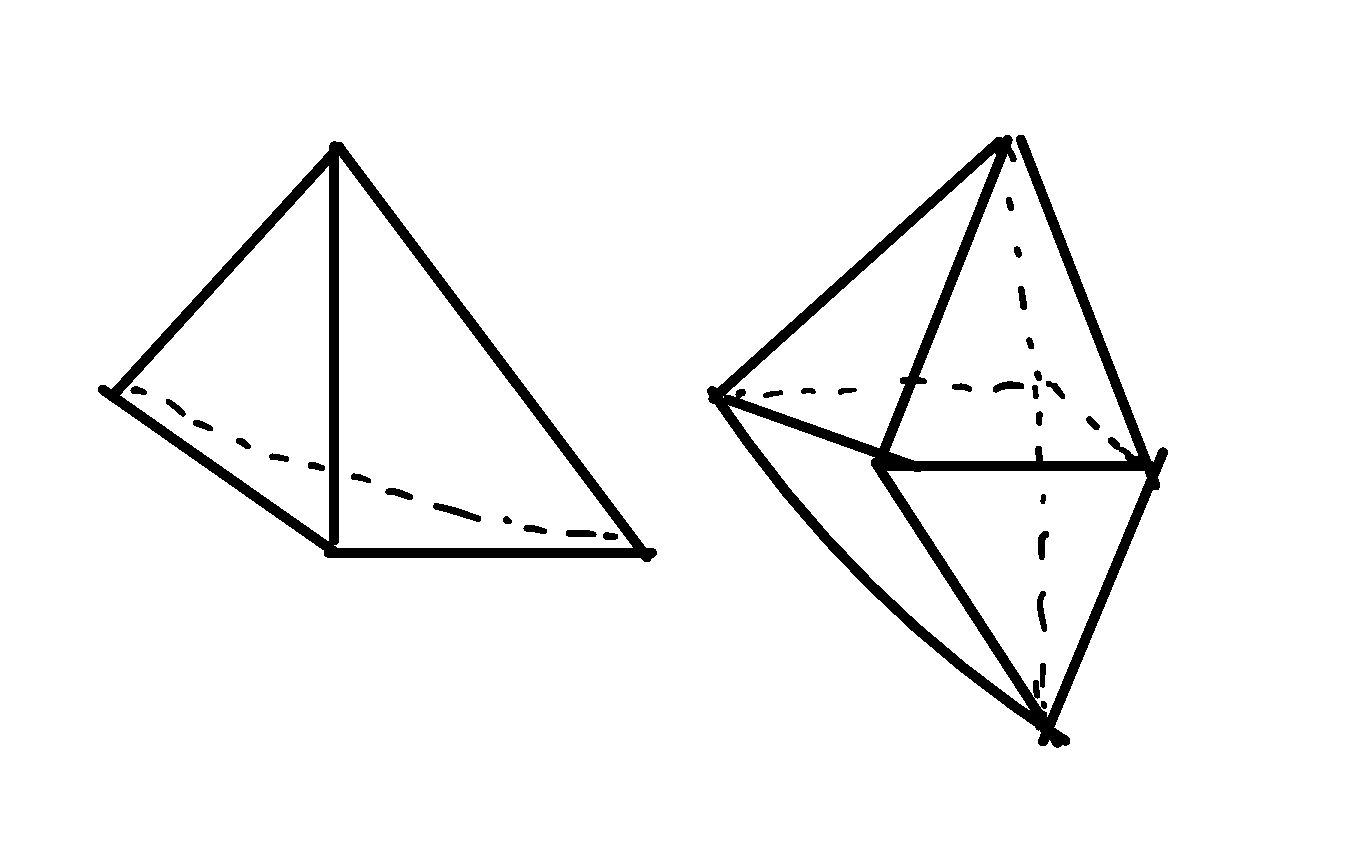
\includegraphics[width=.3\textwidth]{curvature/deltahedron}
\caption{Two deltahedron. A tetrahedron and an octahedron.}
\label{fig:deltahedron}
\end{figure}

How many convex deltahedron are there?
Any convex deltahedron is homeomorphic to the sphere.
So we know $\chi(S)=2$ and there is no boundary.

Let $T=(V,E,F)$  be a triangulation of the sphere.
Here, after scaling by $\pi$ the curvature of a vertex
is $k(v)=4-deg(v).$
Then, the Gauss-Bonnet theorem
states,

$$\sum_{v\in V}K(v)=2\cdot  3\cdot 2.$$
Since we have a triangulation each
vertex must have degree at lease three.
Thus, $k(v)\leq 3$ for all $v$. But, since we have
convex faces, $k(v)\geq 1$ for all $v$.

So, for $1\leq k(v_i)\leq 3$ and  $\sum k(v_i)=12$,
so we only need to examine a finite number (19) of cases.
For example, if the curvature at each vertex is three then,
we have four vertices. Each vertex is incident to three edges
and each edge has two vertices so $\frac{3}{2}4=E=6$ and
there are four faces. This is the tetrahedra.





\section{Triangulating Noncovex Polyhedra}
\label{sec:triangulating}

Discrete three-manifolds are called \EMPH{polyhedra}. 
A polyhedron is \EMPH{simple} if it is homeomorphic to the sphere 
and the faces are all polygons.
Let $P$ be a a simple polyhedron.
A triangulation of a three-manifold is a decomposition
of $P$ into tetrahedra.
Often, we wish to represent the three-manifold
with as few tetrahedra as possible \cite{simplify-mesh-1999}.
Let $n$ be the number of vertices in a simple polyhedron,
in the worst case, decomposing the $P$
 into tetrahedra requires $\Omega(n^2)$ tetrahedra
\cite{chazelle-lower-1984}.

 An edge $e$ in $P$ is
\EMPH{reflex} if the interior angle formed by its two incident faces
is greater than $\pi$.
A vertex is reflex is it is incident to a reflex edge.
Let $r$ denote the number of reflex edges.
See \figref{reflex} for an example.

\begin{figure}[htb]
\centering
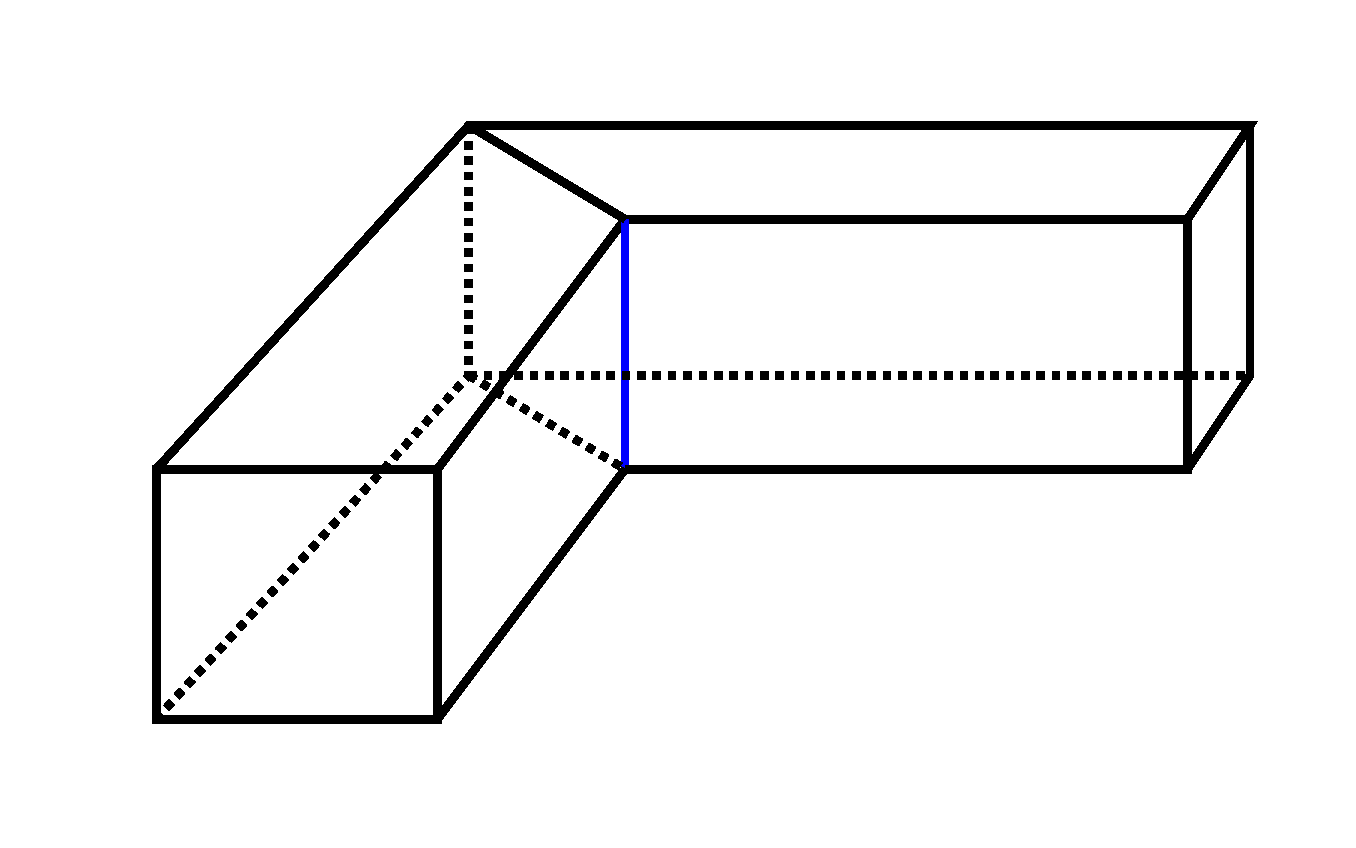
\includegraphics[width=.3\textwidth]{meshes/reflex}
\caption{A polyhedron with one reflex edge (blue), the two vertices incident to the blue
edge are reflex vertices.}
\label{fig:reflex}
\end{figure}
Chazell and Palios give an
algorithm to triangulate a nonconvex simple polyhedra \cite{triangulating-polytope-1990}.
 Their algorithm creates a refinement with $O(n+r^2)$ tetrahedra
in $O(n\log r +r^2\log r)$ time and $O(n+r^2)$ space.
The algorithm first removes $n-4r$ non-reflex or flat vertices
to create a representation of the polyhedra with $O(r)$ vertices.
Then, vertical planes decompose the reduced polyhedra in to
$O(r^2)$ convex cells.

Chazelle and Shouraboura use the Gauss-Bonnet theorem to show any polyhedron
 of genus $g$ must have at least $g-1$ reflex edges~\cite{tetra-bounds-c-s-1994}.
 This implies that any polyhedron
can be decomposed with $O(n+r^2)$ tetrahedra, regardless  of 
the genus!  We present their application.

In this application, to simplify computation we scale the curvature of a vertex
by $\frac{1}{2\pi}$, so be $k_v=\frac{1}{2\pi}\left(2\pi-\sum_i \alpha_i\right)$,
First, we show 

\begin{lemma}\label{lem:reflex-edge}
The number of reflex edges  incident to a vertex $v$  is at least $-k_v.$
\end{lemma}

\begin{proof}

For each vertex, center a sphere at the vertex,
see \figref{sphere-on-vert}.
The intersection of the polyhedron and the sphere
gives a `polygon' on the sphere with boundary $L$ consisting of great
circles. 
Scale the sphere to have unit radius. Then, the length of each arc
in $L$ is equal the the angle incident to $v$, so the total length of $L$ is
the sum of the angles incident to $v$, see \figref{sphere}.

Let $R$ be the number of reflex edges incident to $v$.
If $R$ is zero, then $P$ is convex and has non-negative curvature
so $L\leq 2\pi$. If $R>0,$
reflex edges incident to $v$ correspond to reflex angles in $P$.
If we have a reflex angle in $P$, bisect it and reduce the 
number of reflex angles and obtain a decomposition
of the sphere into at most $R+1$ convex regions,
thus $L\leq 2\pi(R+1)$.

Thus, we have $L=\sum \alpha_f$ and the curvature 
$k_v=2\pi-\sum \alpha_f$ giving
$L=2\pi(1-k_v)$. Combining this with $L\leq 2\pi(R+1)$
gives $-k_v\leq r.$


\end{proof}

\begin{figure}[htb]
        \centering
        \begin{subfigure}[b]{0.35\textwidth}
        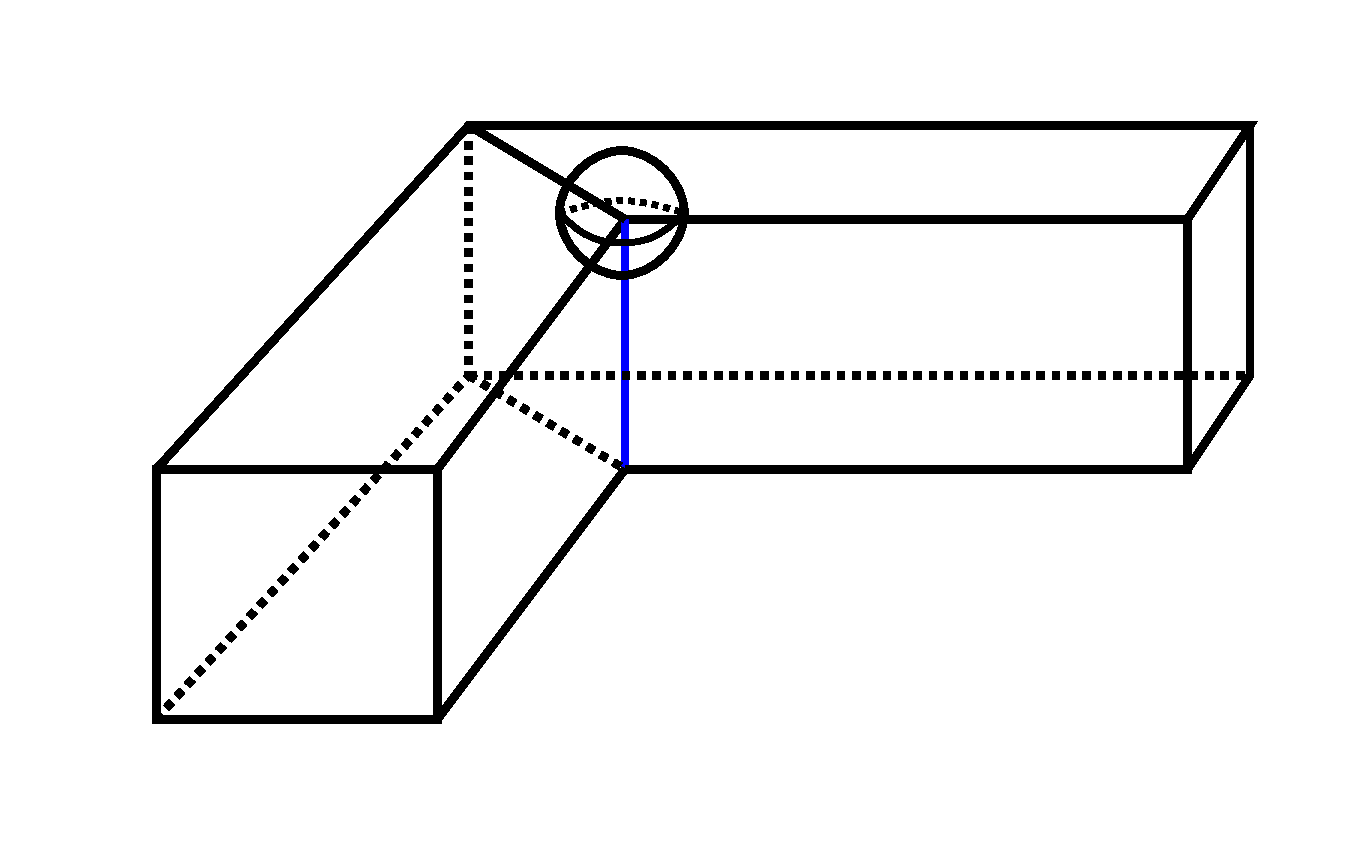
\includegraphics[width=\textwidth]{meshes/reflex-vert-sphere}
        \caption{}
          \label{fig:sphere-on-vert}
        \end{subfigure}
          \hspace{.0cm}
         \begin{subfigure}[b]{0.45\textwidth}
        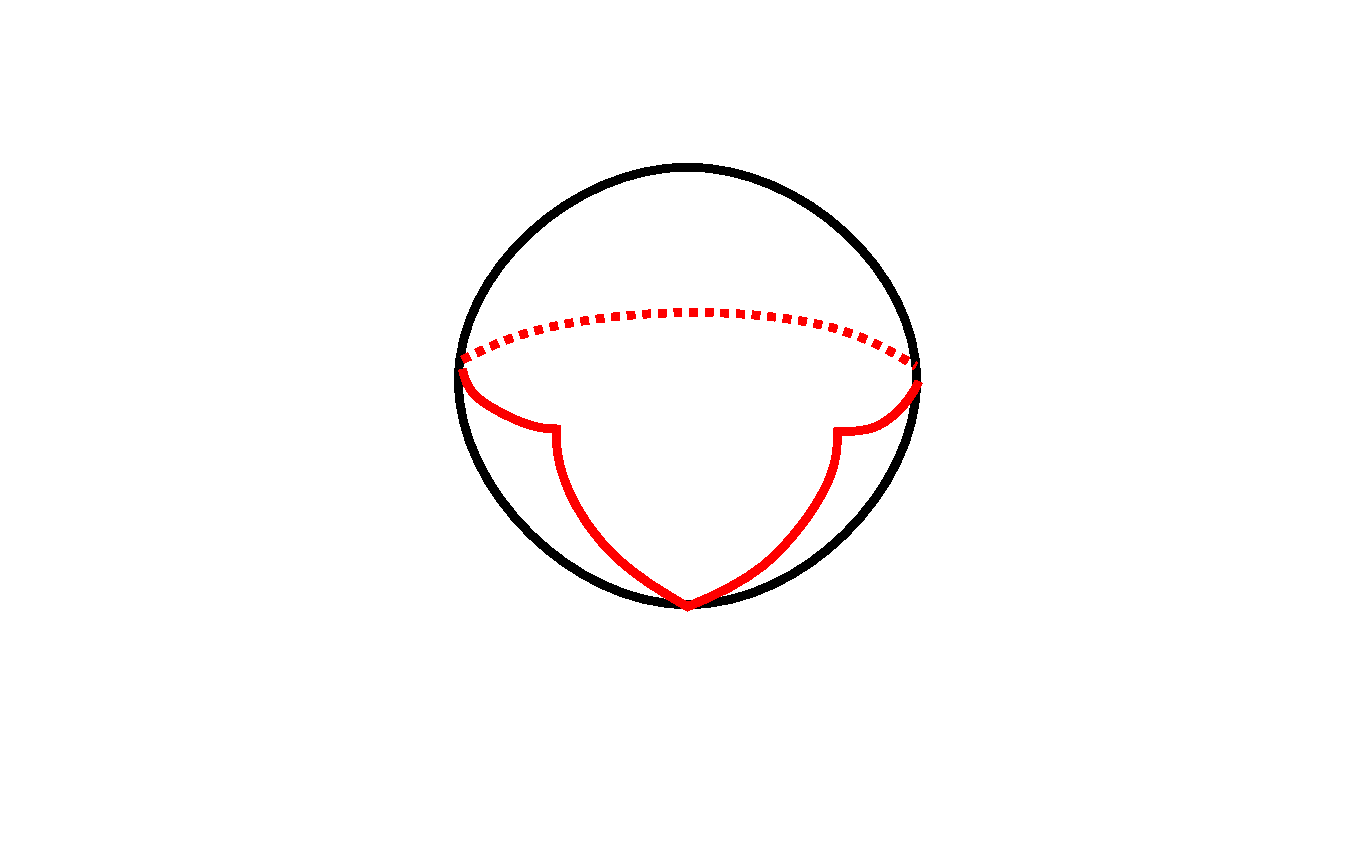
\includegraphics[width=\textwidth]{meshes/sphere-intersection}
        \caption{}
        \label{fig:sphere}
        \end{subfigure}\\
		\caption{(a) A sphere centered at a reflex vertex. (b) The `polygon'
		of great circles where the polyhedron intersects the sphere. 
		\label{fig:sphere}}
\end{figure}


Next, we show
\begin{theorem}[Reflex Angles]\label{thm:reflex}

Any polyhedron of genus $g$ must have 
at least $g-1$ reflex dihedral angles. 

\end{theorem}
\begin{proof}
Let $r$ be the total number of reflex edges in a polyhedra.
By the classification of oriented surfaces, the Euler characteristic 
 is determined by the genus, $\chi=2-2g$.
By \lemref{reflex-edge}, $\sum_v -k_v\leq 2 r$ since each
reflex edge is incident to two vertices.
By the Gauss-Bonnet theorem $\sum_vk_v= 2-2g,$
so $-2r\leq 2-2g$ and $g\leq r+1$ as desired.

\end{proof}

Given a polyhedron of genus $g$, we can temporally 
duplicate the vertices around each essential cycle and insert disks,
 creating a polyhedron of genus zero, we theb apply the algorithm to
decompose genus zero polyhedra given in \cite{triangulating-polytope-1990}.
Then remove the added disks.
Since we added $g$ disks the algorithm decomposes
the polyhedron into $O(n+ (r+g)^2)$ tetrahedra.
By \thmref{reflex}, $g\leq r+1$ showing that the upper bound
on the number of tetrahedra in a triangulation
of a polyhedra is $O(n+r^2)$ regardless of the genus.


\subsection{Digital Topology}
\label{sec:digital-topology}

Digital images consist of arrays of cubes.
Each cube is either black or white.
Given a digital image, one would like 
a computer to to classify the image.
Operations toward image classification include
object counting, border following and computing 
the homology of objects \cite{kong_digital_1989}.
Decomposing a cubical complex into a simplicial complex
results in 24 times as many highest dimensional cells \cite{Kaczynski2003}.


The elements of two-dimensional digital images
are \EMPH{pixels} and the elements of a three-dimensional
digital image are called \EMPH{voxels}.
Each pixel can be associated with a point in a lattice.
Two points in the lattice are four-adjacent if
they are  distinct and differ in at most one of their
coordinates, they are eight-adjacent
if they distinct and each coordinate entry differs by at most one.
In three dimensions, two points
are 26-adjacent if they are distinct and each coordinate 
entry differs by at most one.

If a set of points $S$ lattice points cannot be
partitioned into two subsets that are not
$n$-adjacent is \EMPH{$n$-connected}.

Consider four vertices adjacent to a single vertex $v$.
If four-adjacency is used the four black points are disconnected,
but separate $v$ from the exterior, if eight-adjacency is used
the back points form a Jordan curve that does not separate
an interior. To resolve this matter, we use eight-adjacency
for the white vertices and four-adjacency for the black.
We make a similar choice in three-dimensions.

\begin{figure}[htb]
        \centering
        \begin{subfigure}[b]{0.35\textwidth}
        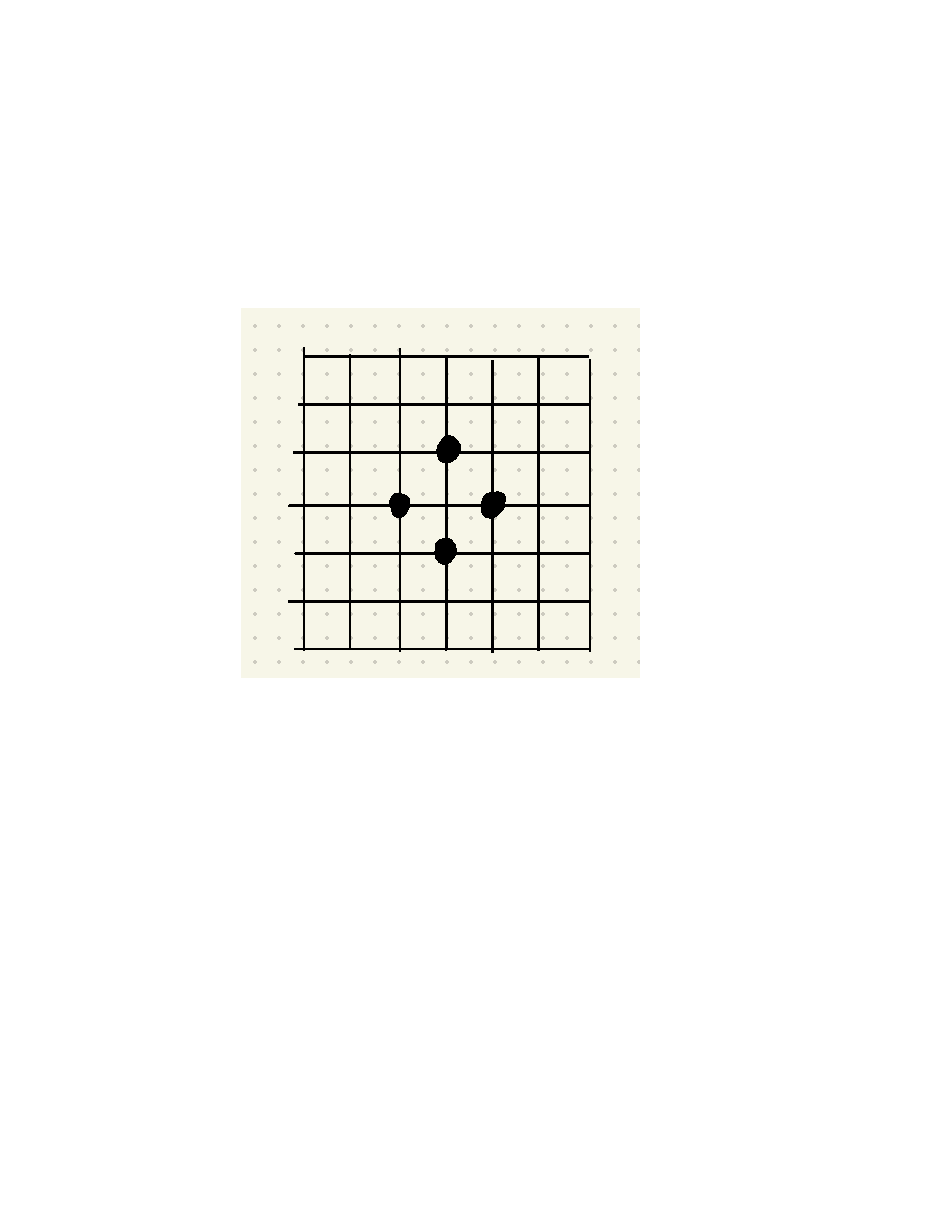
\includegraphics[width=\textwidth]{digital/paradox}
        \caption{}
          \label{fig:paradox}
        \end{subfigure}
          \hspace{.0cm}
         \begin{subfigure}[b]{0.40\textwidth}
        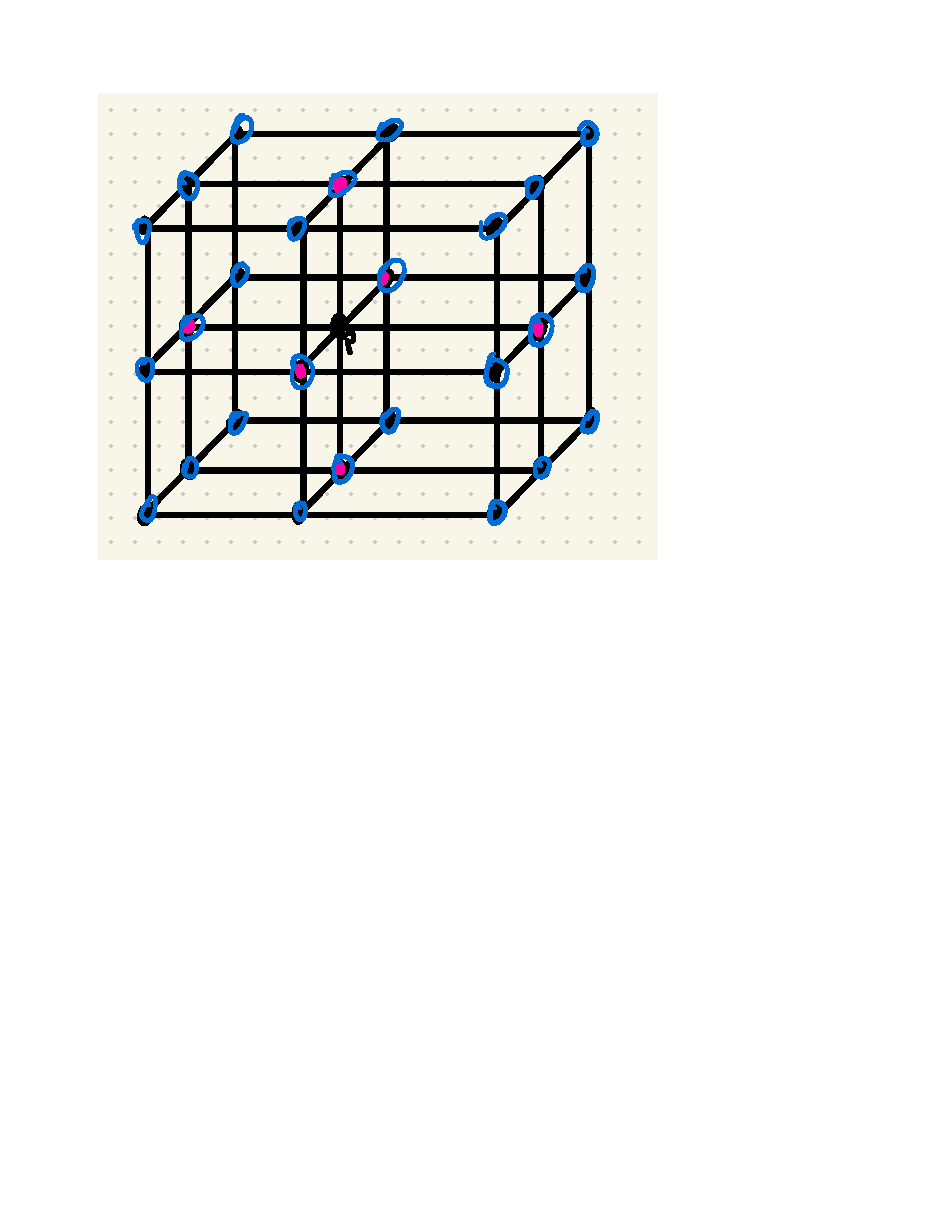
\includegraphics[width=\textwidth]{digital/6-26}
        \caption{}
        \label{fig:6-26}
        \end{subfigure}\\
		\caption{(a) Are the black points a closed curve? (b) In three-dimensions,
		the six neighbors of the vertex $p$ are in pink and the 26 neighbors are in
		blue. 
		\label{fig:adjacency}}
\end{figure}

A \EMPH{digital picture} is a quadruple $(V,m,n,B)$ where
$V=\R^2$ and $(m,n)=(4,8)$ or $V=\R^3$ and $(m,n)=(6,26)$
and $B$ is a subset of $V$. Elements of $B$ are black vertices
and elements not in $V$ are white.

In \cite{chen_digital_2010}, Chen and Rong an
algorithm to compute the homology groups of a three dimensional
digital object in $\R^3$. Their algorithm uses the Gauss-Bonnet theorem
and is linear in the size of the input.


We consider cubical spaces in $\R^3$ with $(6,26)$-connectivity,
where two points are adjacent  if their Euclidean distance is 1.
If $M$ is a closed, orientable digital surface, there are
six types of digital surface points, these are shown in \figref{surface-points}.

\begin{figure}[htb]
        \centering
        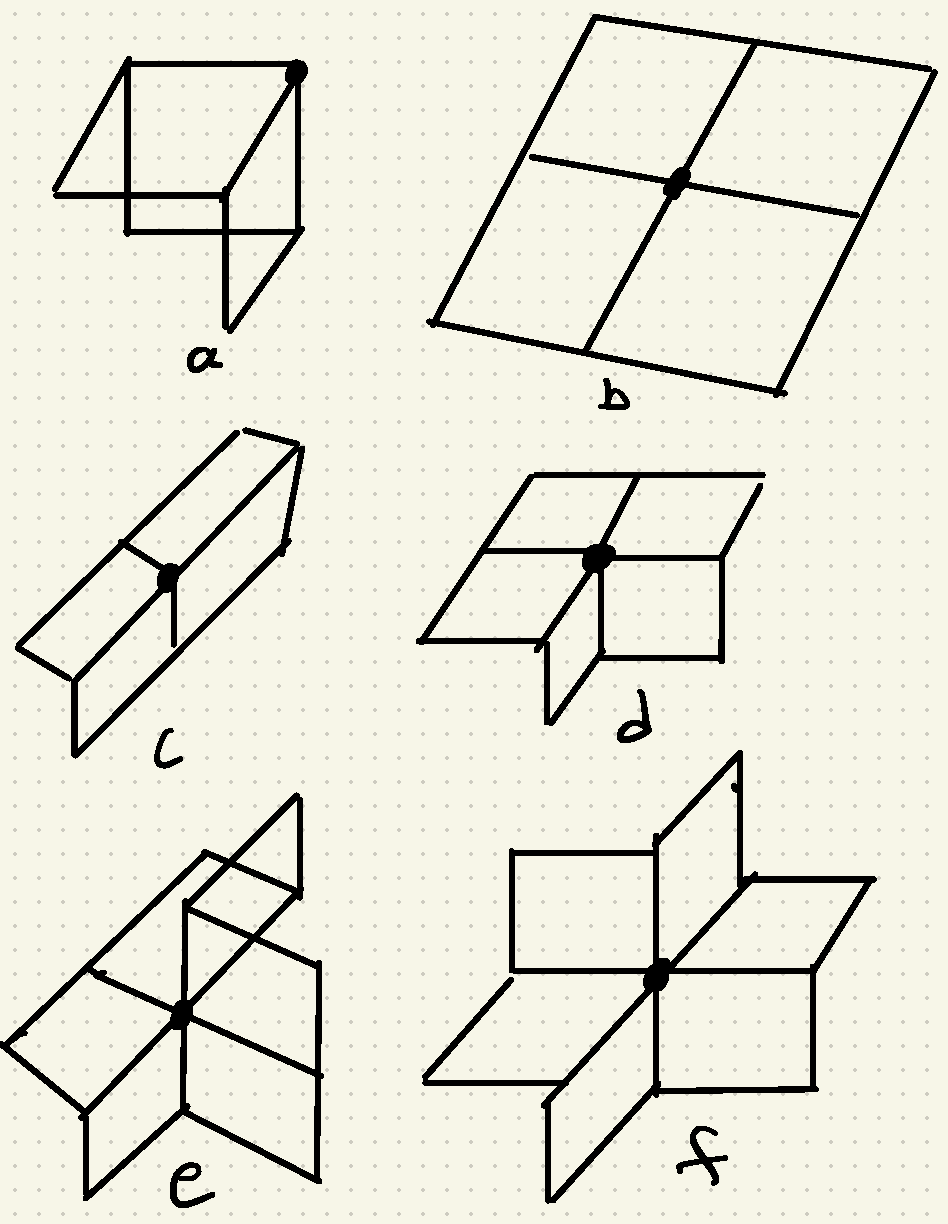
\includegraphics[width=.45\textwidth]{digital/surface-points}
		\caption{
		\label{fig:surface-points}}
\end{figure}

Let $M_i$ denote the set of digital points with $i$ neighbors and $K_i$
the curvature.
Then, by \eqnref{defect}, we have
\begin{enumerate}[(a)]
\item $K_3=\pi/2,$
\item $K_4=0,$
\item $K_5=-\pi/2,$
\item $K_6=-\pi.$
\end{enumerate}

For a closed two-manifold the is the boundary of a three-dimensional
digital image, the Gauss-Bonnet theorem implies
$$\sum_{i=3}^6K_i |M_i|=2(2-2g).$$
A linear time algorithm to compute the genus is the following.
Iterate through all points in $M$ and count the neighbors at each point
and keep track of $M_i$. Then use the above equation to  calculate the genus
using 
$$g=1+(|M_5|+2|M_6|-|M_3|)/8.$$
\section{Homotopy Testing}
\label{sec:homotopy}

Homotopy classes of curves are important  because...
In this section, we share applications
where the Gauss-Bonnet theorem is used to determine
if curve on a surface is contractible.
An explanation of this algorithm is given in a video lecture 
by Jeff Erickson \cite{erickson-lecture}.

\begin{figure}[htb]
\centering
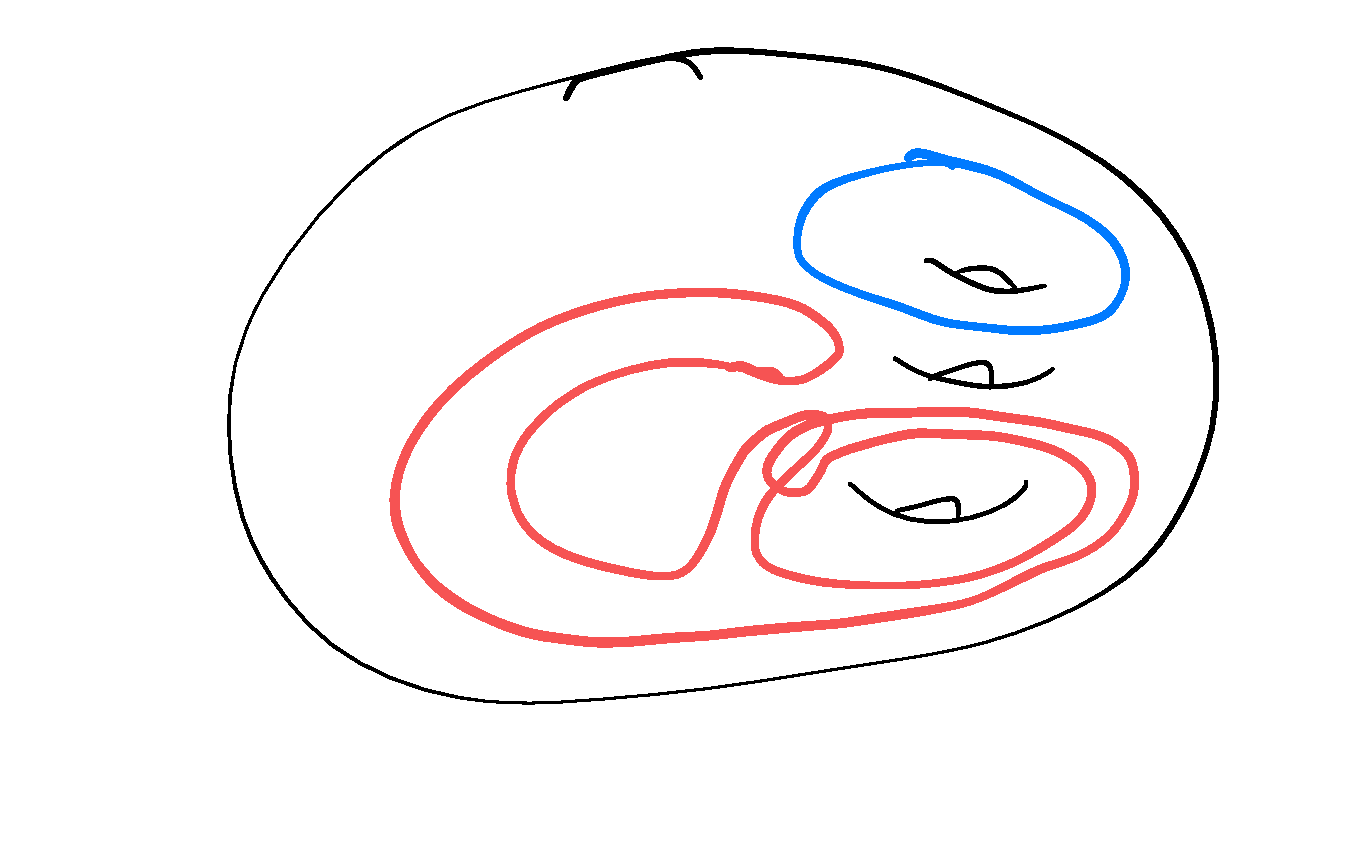
\includegraphics[width=.3\textwidth]{homotopy/contractable}
\caption{The blue curve is not contractable, the red curve is contractable.}
\label{fig:contractable}
\end{figure}

In this application, we will use a modified version
of the Gauss-Bonnet theorem. Given a combinatorial surface
$S$ define the curvature of a face to be $k(f)=1-\sum \beta_f$,
$k(v)=1-\frac{1}{2}\deg(v)+\sum_{v\in V} \alpha_v$.
Summing over all faces and vertices in $S$ gives,
\begin{theorem}[Modified Gauss-Bonnet]\label{thm:modify-g-b}
For a combinatorial surface $S$,
$\sum_{f\in F} k(f)+\sum_{v\in V}k(v)=\chi(S).$
\end{theorem}

\begin{proof}

$$\sum_{f\in F} k(f)+\sum_{v\in V}k(v)=|F|-\sum_{v\in V}\alpha_v + |V|-|E|+\sum_{v\in V}\alpha_v=\chi(S).$$
\end{proof}


Here, a we have a combinatorial surface that we call a map denoted $S$
with genus $g\geq 2.$ The case $g=0$ is the sphere where every curve
is contractible and when $g=1$ contractibility can be determined by a counting
argument\todo{explain}.
A curve is a closed walk, given as alternating sequence of vertices
and edges in $S$.
A \EMPH{homotopy} between two closed curves $\gamma_1$ and $\gamma_2$ that 
share a point $p_0$ is a continuous map $H\colon [0,1]\times \Sp^1 \to \mathbb{R}^2$ 
such that $H(0,\cdot)=\gamma_1$, $H(1,\cdot)=\gamma_2$, and $H(s,0)=p_0=H(s,1)$.

On a combinatorial surface, homotopies can be decomposed
into discrete moves called edge spikes, edge unspikes  and face flips.
The question we consider is: Given a closed walk $W$ in a map $\Sigma$ is there a finite
sequence of moves that reduces the curve to a trivial walk?


First, we transform $S$ into a simpler object called a system of loops.  
Let $T$ be a spanning tree of $S$, let $C$ be the edges in a co-tree
(a spanning tree of the dual), and let $L$ denote the left over edges,
Each edge in $S$ is in one of $(T,L,C)$.
Contract edges in $T$, delete edges in $C$ a system of loops $\Delta$.
When we contract and delete edges in $S$ we might affect edges in our walk $W$.
If we contract an edge in $W$, delete the edge from $W$.
If we delete and edge $e\in W$, face flip to avoid the deleted edge.
Get a new walk $W' \in \Delta$ homotopic to $W\in \Sigma$
now only haveing one vertex. Then, $W'$ has one vertex
with degree $4g$, one face with $4g$ edges, and $2g$ loops.
The length of the walk increases by at most $2g$.


The universal covering space of $S$ denoted $U$ is a plane
and when $g\geq 2$ $U$ has a natural hyperbolic geometry,
tiled by $4g$-gons.


Big idea: a curve is contractible closed walk in $S$
if and only if the walk is closed $U$.
Thus, our problem is equivalent to the following: Given a walk
in the universal cover of a system of loops, is it closed?

Here the walk is given as a starting vertex then we have a list of which
edges to take at each intermediate vertex. 
All vertices look the same, so we must determine if we have ended where
we began. 

Look for spurs or taking and instances where we talk the long way around a face, 
shorten the walk.
Any nontrivial contractible cycle contains either a spur or a bracket \cite{gertsen-short-1990}.
\begin{lemma}[Dehn's Lemma]\label{lem:dehn}
If $g\geq 2,$ then any nontirival closed walk has either a spur
or $4g-2$ consecutive edges on the boundary of a face.
\end{lemma}
\begin{proof}
Sketch: 
Any nontrival closed walk bounds a disk $D$ with $\chi(D)=1$, by the Gauss-Bonnet theorem
$$\sum_v k(v)+\sum_f k(f) =1.$$

Each face has $4g$ edges, each internal vertex has degree $4g$
and each  boundary vertex  has degree less than $4g$.
The angle of each angle on a face  is $\frac{1}{4}$,
thus, $k(f)=1-g<0,$ for internal vertices  $k(v)=1-g<0$ and for all
vertices on the boundary, $k(v)=\frac{3}{4}-\frac{\deg(v)}{4}$.
Boundary vertices fall into three  categories: convex, where $k(v)=\frac{1}{4}$
flats,  where $k(v)=0$  and concave where $k(v)<0$.

By G-B, $$|F|(1-g)+|v_{convex}|\frac{1}{4}\geq 1$$
and 
$$|v_{convex}|\geq (4g-4)|F|+4.$$

We divide by $|F|$ to determine the average number
of convex vertices per face to be greater than $4g-4$.
Thus, there exists some face that has $4g-3$ consecutive edges in the walk.
\end{proof}

This gives an algorithm for determining if a walk is closed in the universal
covering space.
Look for spurs and long boundary subpaths, the walk is closed if and  only if
we can  shrink the curve.
Label edges, walk is a sequence of labels
look at intervals of $4g-2$ in a walk, $8g$ paths
that represent long boundary paths, $4g$ spurs.
Slide window and look for spurs or long boundary paths.
If you find one remove it.

Brute force $O(g^3\ell)$ overall.
Can speed it up with Erickson DFA  idea
$O(g^2+g\ell)$.
Overall runtime $O(n+g^2+g\ell)$ time.

In trouble if $g$is big. Erickson uses system of quads,
radial map, $O(n)$ runtime  \cite{erickson-whittlesey-2013}.






\input{body/fta}


{
\small
\bibliographystyle{abbrv}
%\bibliographystyle{plainurl}
\bibliography{references}
}
\end{document}

